\section{Preliminaries}\label{sec:preliminiary}
\handan{}{should we have this section before properties section? If prop section comes after this section we should remove some descriptions of entities in the properties section e.g., validator, fisherman}
\eray{}{-comment: I agree. I think it may help the reader understand the properties better after reading the design.-}
\begin{figure}[h]
	\centering
	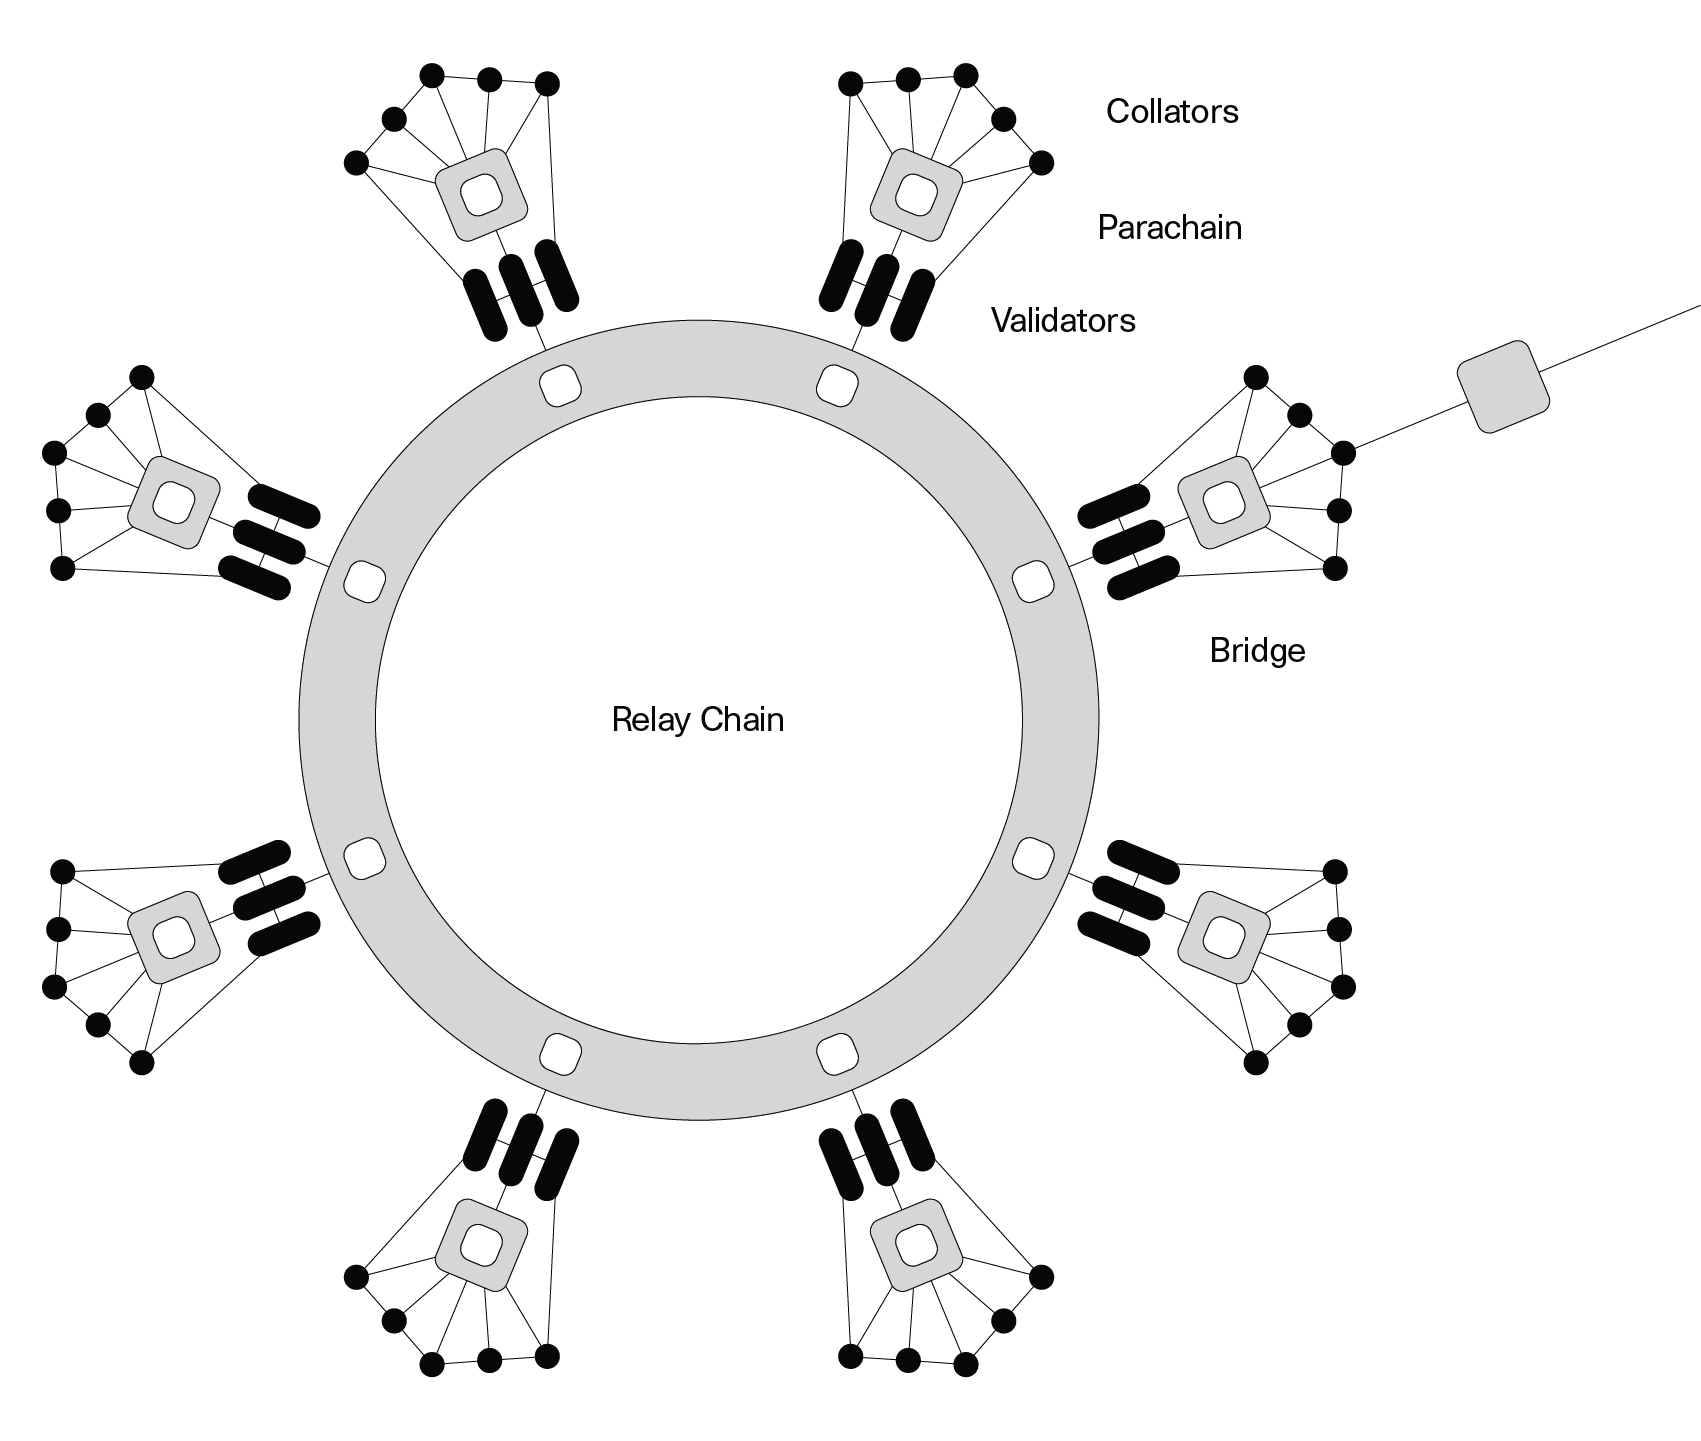
\includegraphics[width=.7\textwidth]{images/Network@2x.png}
	\caption{Polkadot network structure showing relay chain and parachain and including the roles collator, validator (Image credit: Ignasio Albero)}
	\label{fig:roles}
\end{figure}
\subsection{Structural elements of Polkadot}
Next, we review the structural elements and roles, shown in Figure~\ref{fig:roles}, that are defined for the Polkadot protocols.
\paragraph{Parachains:} Multiple heterogeneous blockchains run in parallel in Polkadot.

\paragraph{Relay Chain:} This is a central chain in Polkadot. It keeps references
to all canonical parachain blocks, and thus works as a single source of truth across parachains.
It also keeps references of all cross-parachain messages.

\subsection{Roles}

\paragraph{Validators:} A fixed set of actors called validators are responsible to maintain the relay chain
and keep its consensus, and by extension, maintain the consensus of all the parachains.
In addition, at regular intervals validators are divided into random disjoint subsets
that are each assigned to a particular parachain.
Each of these validator subsets ensures the validity and availability of its parachain's blocks.
Validators receive regular remunerations in DOTs,
and are likewise heavily staked and prone to slashing in case of offenses.

\paragraph{Nominators:} The role of validator is \eray{permissionless}{-comment: I do not understand what is meant by permissonless.-}
 (like all roles in Polkadot),
but the number of slots for validators is limited. Hence, validators must be elected by the community.
In particular, any DOT holder may assume the role of a \emph{nominator}, lock some stake, and publish a list
of trusted validator candidates. Candidates with the most nominators' support get elected,
and nominators share the economic rewards, or slashes, of their supported validators.
Having nominators allows for an unlimited amount of actors and DOTs to participate in the security of Polkadot.

\paragraph{Collators: } Every parachain has its own set of full nodes called collators.
A collator produces new blocks and sends it to the \handan{parachain-assigned validators}{why not just parachain validators?}.
It may only build on top of the parachain blocks that are referenced in the relay chain.
Collators also process outgoing and incoming cross-chain messages.

\paragraph{Fishermen:} Fishermen are staked actors that run background checks on the performance of validators.
In particular, they raise reports in case that a validator-approved parachain block is unavailable or invalid.
They are rewarded for correct reports, and slashed for bogus ones (which helps avoid report spamming).




\subsection{Adversarial Model of Polkadot}

%The adversarial assumption on collators depends on the parachain type. If the parachain is private,
%we assume that there is at least one honest collator.
%Otherwise, we assume that at least the majority of collators are honest.
\paragraph{Parties} In Polkadot, honest parties follow the protocol while malicious ones can follow any arbitrary algorithm. We assume that less than one third of the validators are malicious. On the other hand, we do not have any limit on number of malicious fishermen.
%TODO: What about nominators and collators 

\paragraph{Parachains:} %TODO after session about parachain strategies.

\paragraph{Keys:} We assume that malicious parties generate their keys with an arbitrary algorithm
while honest ones always generate their keys securely. 

\paragraph{Network and Communication:} All validators have their own local clock and their clocks do not rely on any central clock.
We assume that  validators and collators are in a partially synchronous network.
It means that a message sent by a validator or collator arrives at all parties in the network
at most $\D$ units of time later where $\D$ is an unknown parameter. So, we assume an eventual delivery of a message in Polkadot.
We also assume that collators and fishermen can connect to the relay chain network to submit their reports.
%TODO: Do we have authenticated channel between validators?
